\subsection{Connected shared-adapter reasoning results}
The completed automatic comparison links exported FedAvg and FLEN shared adapters to the same inference protocol as the base checkpoint. Table~\ref{tab:revision-agents} compares role prompting with one-call prediction and four-call self-refinement. These are paired case outcomes for seed-41 checkpoints. Legal soundness, coherence, preference and unsupported-claim rates await completed independent blinded review sheets.

\begin{table}[t]
\caption{Sixty paired reasoning cases per checkpoint. Differences are four-stage minus single-agent accuracy in points; intervals use paired case bootstrap. The four-stage comparator is regenerated deterministically across call-budget packages and counted once.}
\label{tab:revision-agents}
\centering
\small
\resizebox{\linewidth}{!}{%
\begin{tabular}{lrrrrrr}
\toprule
Checkpoint & Single calls & Single (\%) & Four-stage (\%) & Difference & 95\% CI & McNemar $p$ \\
\midrule
base & 1 & 21.7 & 15.0 & $-6.7$ & $[-16.7,3.3]$ & 0.344 \\
base & 4 & 18.3 & 15.0 & $-3.3$ & $[-13.3,6.7]$ & 0.754 \\
federated & 1 & 5.0 & 20.0 & $+15.0$ & $[5.0,25.0]$ & 0.012 \\
federated & 4 & 20.0 & 20.0 & $+0.0$ & $[-5.0,5.0]$ & 1.000 \\
flen & 1 & 1.7 & 25.0 & $+23.3$ & $[13.3,35.0]$ & $<0.001$ \\
flen & 4 & 18.3 & 25.0 & $+6.7$ & $[0.0,15.0]$ & 0.219 \\
\bottomrule
\end{tabular}
}
\end{table}


The one-call FedAvg and FLEN controls parse successfully on only 14 and 10 of 60 cases, respectively. Their large four-stage gains therefore combine task accuracy and output-format compliance. Four-call self-refinement raises successful parsing to 58 and 59 cases. Against that control, four-stage accuracy changes by 0.00 points for FedAvg and 6.67 points for FLEN (95\% paired bootstrap interval $[0.00,15.00]$; exact McNemar $p=0.219$). The base checkpoint decreases by 3.33 points. These call-matched results leave the reasoning advantage uncertain.

\begin{table}[t]
\caption{Output-format diagnostics on 60 cases. S denotes single-agent prediction and D four-stage deliberation. Conditional accuracy (percent) uses only cases parsed in both conditions and is descriptive; primary accuracy retains all cases and counts parsing failures as errors.}
\label{tab:revision-agents-parse}
\centering
\small
\resizebox{\linewidth}{!}{%
\begin{tabular}{lrrrrrr}
\toprule
Checkpoint & Single calls & Parsed S & Parsed D & Both & Cond. acc. S & Cond. acc. D \\
\midrule
base & 1 & 58 & 55 & 53 & 18.9 & 17.0 \\
base & 4 & 58 & 55 & 54 & 16.7 & 16.7 \\
federated & 1 & 14 & 60 & 14 & 21.4 & 14.3 \\
federated & 4 & 58 & 60 & 58 & 20.7 & 19.0 \\
flen & 1 & 10 & 59 & 10 & 10.0 & 10.0 \\
flen & 4 & 59 & 59 & 58 & 19.0 & 24.1 \\
\bottomrule
\end{tabular}
}
\end{table}


\begin{table}[t]
\caption{Mean analysis cost per case with four calls in both conditions. The common presentation step is excluded; call matching does not match token consumption.}
\label{tab:revision-agents-cost}
\centering
\small
\resizebox{\linewidth}{!}{%
\begin{tabular}{lrrrr}
\toprule
Checkpoint & Protocol & Prompt tokens & Generated tokens & Seconds \\
\midrule
base & Self-refinement & 1942.7 & 96.7 & 1.68 \\
base & Four-stage & 2711.1 & 447.5 & 7.69 \\
federated & Self-refinement & 2074.6 & 251.0 & 5.70 \\
federated & Four-stage & 2635.5 & 375.6 & 8.51 \\
flen & Self-refinement & 2081.5 & 256.4 & 6.43 \\
flen & Four-stage & 2601.0 & 360.2 & 8.93 \\
\bottomrule
\end{tabular}
}
\end{table}


For the FLEN checkpoint, four-stage analysis consumes 360.3 generated tokens and 8.93 seconds per case, compared with 256.4 tokens and 6.43 seconds for self-refinement. The extra deliberation therefore increases generated tokens by about 41\% and observed elapsed time by about 39\%.

\begin{figure}[t]
\centering
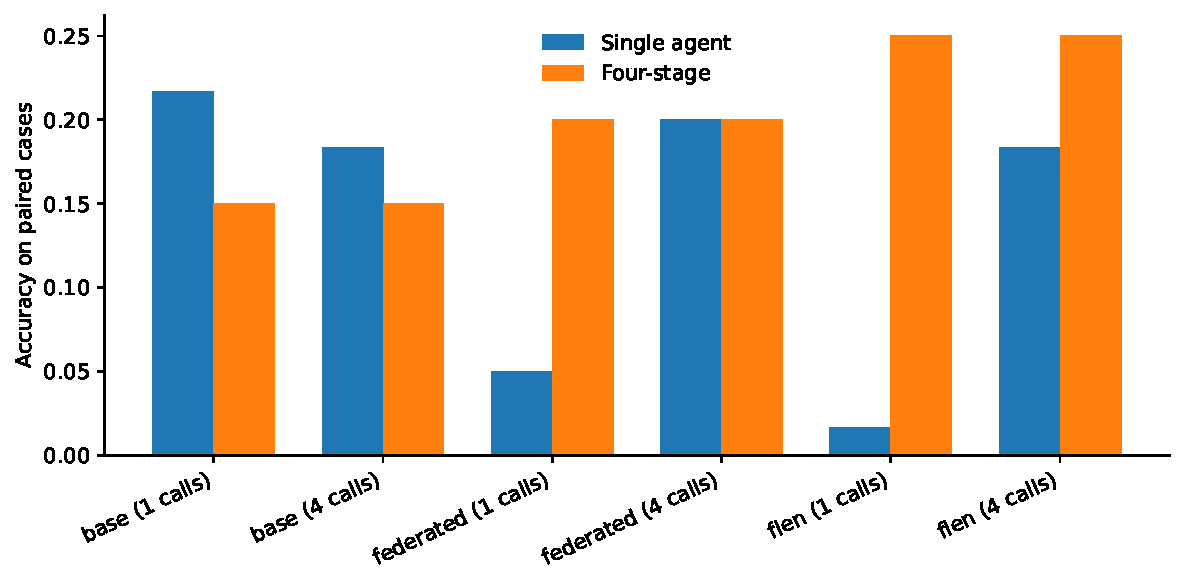
\includegraphics[width=\linewidth]{revision_agents.pdf}
\caption{Automatic paired accuracy with base, FedAvg shared and FLEN shared checkpoints; call budgets label the single-agent controls.}
\label{fig:revision-agents}
\end{figure}
